%!TEX root = ../../main.tex

\chapter{Data Preprocessing}

Based on \cite{football-predictor} five sliding windows for match data were implemented. The idea of these sliding windows is to deliver match data in historical order and to aggregate data on a team's performance during the last 10 games.
First the relevant data was extracted in chronological order with the following SQL statement:

\begin{lstlisting}[language=SQL, caption=SQL code for Sliding Window]
SELECT id, country_id, league_id, season, date, home_team_api_id, away_team_api_id, home_team_goal, away_team_goal, B365H, B365D, B365A, shoton, shotoff, possession
FROM Match
ORDER BY date asc
\end{lstlisting}

Since the bookkeeper odds are highly correlated, as has been pointed out in \autoref{chap:data_understanding}, only Bet365 data (B365H = odds home team wins, B365A = odds away team wins, B365D = odds draw) will be used.


\section {Slliding Windows or Data Options}

\subsection {Option 1}
For the first sliding window or option, data on shoton, shotoff and possession are not necessary and therefore are dropped. Moreover, rows without odds are dropped as well. The resulting data is saved as a CSV file:


\begin{lstlisting}[language=Python, caption=Python code for matches\_all.csv]
conn = sqlite3.connect("../data/eusoccerdatabase.sqlite")
query = "SELECT id, country_id, league_id, season, date, match_api_id, home_team_api_id, away_team_api_id, home_team_goal, away_team_goal, B365H, B365D, B365A, shoton, shotoff, possession FROM Match ORDER BY date asc"
df = pd.read_sql_query(query, conn)
df = df[np.isfinite(df['B365H'])] # drop rows without odds
df_noxml=df.drop(['shoton', 'shotoff', 'possession'], axis=1)
df_noxml.to_csv("../data/matches_all.csv")
\end{lstlisting}

This CSV file consists now of 22592 rows each representing one football match including information on how many goals each team scored, what the odds were and the date of the match:

\begin{figure}[H]
\begin{center}
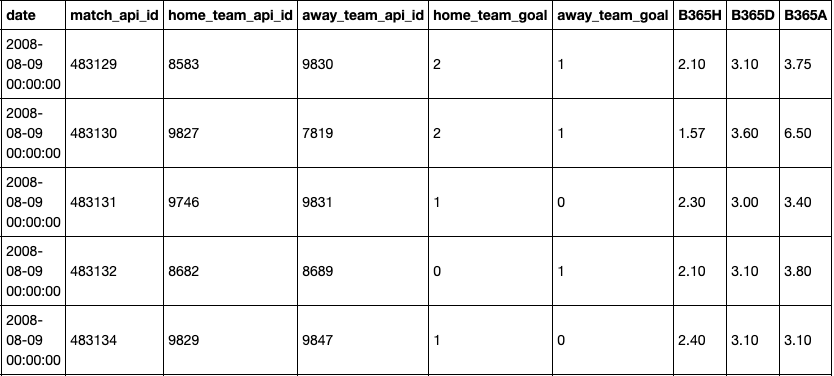
\includegraphics[scale=.55]{matches_all_csv.png}
\end{center}
\caption{Data for Option 1}
\label{fig:matches_all_csv}
\end{figure}

This CSV file was then used for the first sliding window. The code for it \cite{sliding01} expects a CSV file and processes it row by row. For every match the outcome of the game based on scored goals is calculated. Moreover, statistics on how each of the two opponents performed in the previous ten games are generated:

\begin{figure}[H]
\begin{center}
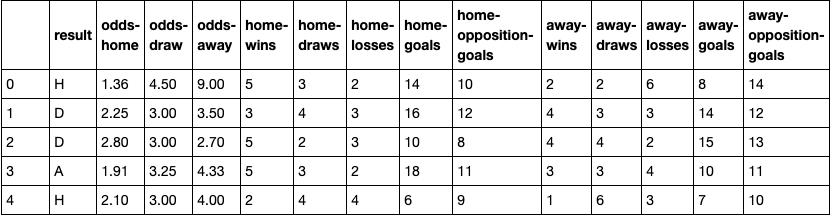
\includegraphics[scale=.55]{sliding_window_option1.png}
\end{center}
\caption{Sliding Window Option 1}
\label{fig:sliding_window_option1}
\end{figure}

As an example we can see in row 0 that the home team won, which is indicated by a capital "H". The odds that the home team wins were 1.36, 4.50 for a draw and odds of 9.0 that the away team wins. In the last 10 matches the home team won 5 times, finished 3 matches with a draw, lost 2 times and scored 14 goals. Opposing teams were able to score 10 goals. Subsequent columns contain the equivalent statistics for the opposing/away team. The first sliding window reduces the total dataset to 20823 rows and generates 13 features. Furthermore, now 3 distinguishable classes (H = home team wins, A = away team wins, D = draw) are available.


\subsection {Option 2}
This option, which uses a slightly enhanced version \cite{sliding02} of the first sliding window code, adds statistics on goal shots:

\begin{figure}[H]
\begin{center}
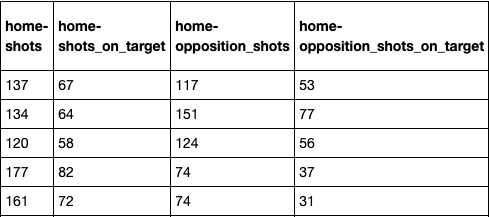
\includegraphics[scale=.55]{sliding_window_option2.png}
\end{center}
\caption{Sliding Window Option 2}
\label{fig:sliding_window_option2}
\end{figure}

Unfortunately due to the poor choice of data origin this option reduces the dataset to 7033 rows. But on the bright site, this option extends the number of features to 21.

\subsection {Option 3}
Based on option 2, option 3 additionally calculates shot accuracy statistics with code written and executed in a Jupyter Notebook \cite{jupyter_sliding}:

\begin{figure}[H]
\begin{center}
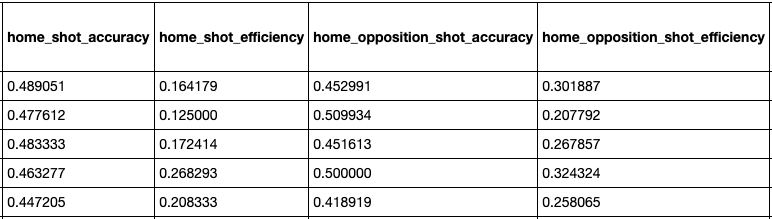
\includegraphics[scale=.55]{sliding_window_option3.png}
\end{center}
\caption{Sliding Window Option 3}
\label{fig:sliding_window_option3}
\end{figure}



Option 3 has 29 features and 7033 rows. "x\_shot\_accuracy" represents the percentage of the shots which actually hit the goal or goal keeper and "x\_shot\_efficiency" the percentage of the shots which actually were counted as goals.


\subsection {Option 4}

Option 4 again uses an enhanced enhanced version \cite{sliding04} of the first sliding window code and extends option 2 with ball possession statistics:

\begin{figure}[H]
\begin{center}
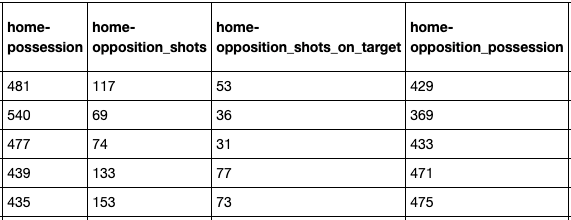
\includegraphics[scale=.55]{sliding_window_option4.png}
\end{center}
\caption{Sliding Window Option 4}
\label{fig:sliding_window_option4}
\end{figure}

Ball possession is provided in minutes. This option has 6996 rows and 25 features.

\subsection {Option 5}
The last option is based on option 3 and additionally includes ball possession statistics. It has the highest number of features (33) and 6996 rows. The Python code for it can be found in the same Jupyter Notebook as for option 3 \cite{jupyter_sliding}.


\section {Data Profiling Part 2}

Using Pandas Profiling all sliding windows or options were profiled again. Here is and excerpt of the profile for option 3:

\begin{figure}[H]
\begin{center}
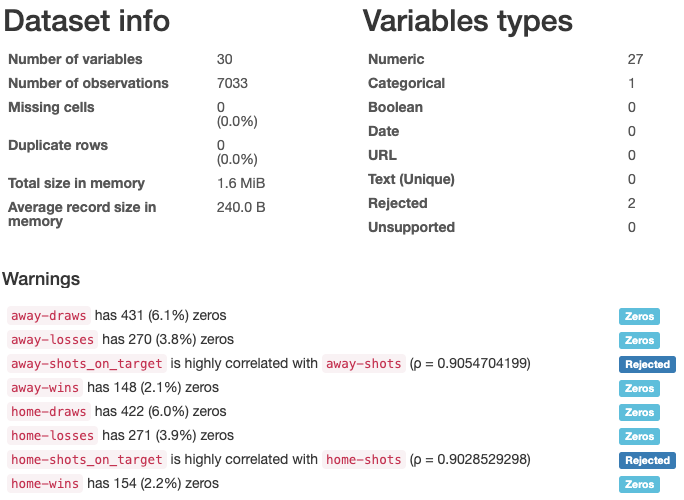
\includegraphics[scale=.6]{profiling_option3.png}
\end{center}
\caption{Pandas Profiling Sliding Window 3}
\label{fig:profiling_option3}
\end{figure}

Apart from one variable, which holds the classes respectively the outcome H, A, or D of a football match, all features/columns are numerical and no values (cells) are missing now. As expected x-shots and x-shots\_on\_target are highly 
correlated. Interestingly zero values are marked as warnings. However, in this context they are fine and still usable. Without having doming knowledge and purely relying on tools, one might be inclined to drop these values and lose valuable information. Another interesting information found in Pandas profiles is the total size in memory. 1.8 MiB shows that the data for option 3 is little and definitely small enough to fit into RAM or GPU Memory. This information is valuable, as will be shown later.
\newline
Since the profiles for the other options are similar to the one described above, they will not be explained.

\section {Normalization}
Since the input data varies in scale it has to be normalized, except the "result" column which has to be encoded. Normalization is the process which normalizes all input data avoiding negative effects in regards to decisions of a neuron. 
The following lines of code normalize the data in a dataframe:

\begin{lstlisting}[language=Python, caption=Python code for normalization]
from sklearn import preprocessing

column_names_to_not_normalize = ['result']
column_names_to_normalize = [x for x in list(dataframe) if x not in column_names_to_not_normalize ]
x = dataframe[column_names_to_normalize].values
x_scaled = preprocessing.normalize(x)
df_temp = pd.DataFrame(x_scaled, columns=column_names_to_normalize, index = dataframe.index)
dataframe[column_names_to_normalize] = df_temp
\end{lstlisting}


\section {Encoding}

The classes H,A,D respectively the outcome of football match which shall be predicted, have to be encoded before they can be used. Using sklearn this can be achieved with only a few lines of code:

\begin{lstlisting}[language=Python, caption=Python code for encoding classes]
from sklearn import preprocessing

le = preprocessing.LabelEncoder()
le.fit([ "H", "A", "D"])
dataframe.loc[:,['result']]=le.transform(dataframe['result'])
\end{lstlisting}


\section {Functions and Input Data For Neural Networks}
The repetitive data preparation tasks encoding, normalization, splitting data into training and test data as well as getting data and prediction labels have been solved using Python functions. Furthermore, Pandas dataframes cannot be used as input for neural networks written with Tensorflow and Keras. The complete code, which has been partly described above, can be found here \cite{colab_nn}.
\newline
Since the data for all options is very little and fits completely into RAM, as has been described above, no input functions for Tensorflow models, e.g. neural networks, had to be written. An excerpt of how the final input data as numpy array for the neural networks described in \autoref{cha:Modelling} looks like can be seen here:

\begin{figure}[H]
\begin{center}
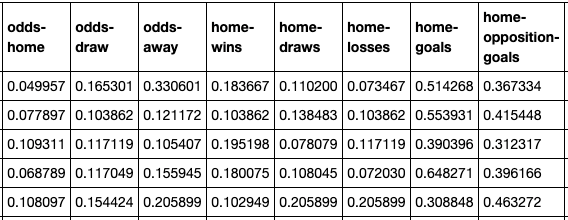
\includegraphics[scale=.6]{input_data.png}
\end{center}
\caption{Excerpt of Input Data for Neural Networks as Numpy Array}
\label{fig:inpud_data}
\end{figure}














